This chapter presents a deep analysis of the dataset used. On section one an overall description
and main statistics are shown. Section two consists of an early analysis of the data along with
the preprocessing steps taken. Finally section 3 makes an analytical definition of the problem
of learning urban perception from this data.


\section{Description}
As was mentioned previously, this work is based on the Place Pulse 2.0 dataset \cite{hidalgo_placepulse}.
PP 2.0 is a crowdsourced dataset designed for learning urban perception from street view like images.
Unlike regular datasets for supervised machine learning, that have labels for each image, Place Pulse
consists of pairwise comparisons between images, and the ground truth is a vote representing which of
the images is more representative of an attribute (ties are also possible). That structure makes
traditional classification / regression approaches inapplicable, but opens the door for
pairwise based ranking techniques, that are more suitable to urban perception since a ground truth for
how much an image represents an abstract attribute such as "safety" it's impossible to define.

The dataset consists of approximately 1.2 million pairwise comparisons of 112,000 images from 56 cities,
distributed on 6 attributes: wealthy, safety, depressing, boring, lively and beautiful, making it
the biggest available dataset for urban perception. The crowdsourcing survey was
active for 5 years and it was answered by 81,630 different users. Demographic information
about the users was not collected.

One of the main issues with PP 2.0 is that the authors made only the votes available,
supplying only the geographical coordinates of the images, so that they can be downloaded from
the google street view API, but changes in the API interface and the available images through out
the years have made it increasingly difficult and costly to download the original dataset for
new researchers.

\section{Analysis and preprocessing}

As a first preprocessing step all noisy images are removed by using a size threshold,
since images small in size are mostly  google api errors or unintelligible places like
dark tunnels.

Is important to note that, unlike most crowdsourced datasets, the authors of PP didn't
do any validation on the votes by making it so that the same question was answered by more than
one person, and deleting inconsistent votes. 99.59\% of the image pairs that appear in the
data set have a single vote in a category (see \ref{fig:rep_hist} for details.), making it impossible to validate them in any way.
Even though some research indicates that answers to this surveys aren't affected by user
bias or demographics \cite{hidalgo_inequality, costa_lisbon}, the noise in the votes is a
clear dataset disadvantage. 34\% of the  pairs that have more than one vote in an attribute
show inconsistencies between the votes.


\begin{figure}[ht]
	\begin{center}
	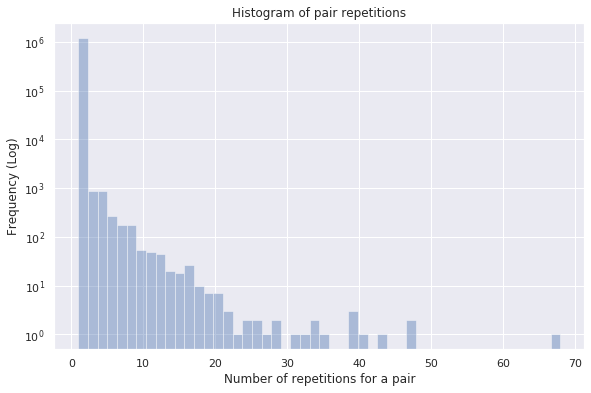
\includegraphics[width=0.8\textwidth]{./figures/rep_hist.png}
	\caption[Repetition histogram]{ Histogram for amount of repetitions for each pair of images }
	\label{fig:rep_hist}
	\end{center}
\end{figure}

For this work all the inconsistent duplicates are removed and a single vote of those consistent is kept
in the dataset. After this steps 1,207,938 votes for 111,299 images are left. See table \ref{tab:votes}
for the exact vote distribution.

\begin{table}[H]
	\begin{center}
	\caption[Votes Distribution]{ Vote distribution after preprocessing.}
	\begin{tabular}{ll}
		\hline
		\textbf{Attribute} & \textbf{\# of votes} \\ \hline
		Wealthy            & 150,370               \\
		Safety             & 364,130               \\
		Depressing         & 130,781               \\
		Boring             & 125,744               \\
		Lively             & 263,123               \\
		Beautiful          & 173,790               \\ \hline
		Total              & 1,207,938            \\
	\end{tabular}
	\label{tab:votes}
	\end{center}
\end{table}

Users of the survey had the possibility of voting that a pair is tied for an attribute,
meaning that they didn't perceive any significant difference, previous works just
discard this data and don't use it for learning, focusing only on the votes where a winner was
chosen \cite{hidalgo_placepulse,zhang_measuring,tamara_judgments}. After preprocessing 15.3\% of the
votes are ties, which means a significant amount of information is lost by disregarding them.


\section{Problem Definition}

Following a similar formulation than \citeA{hidalgo_placepulse}, each attribute $A$ in the PP 2.0 dataset consists of a set
of $m$ images $I_A = \{x_i\}_{i=1}^m \in \mathbb{R}^{h \times w \times 3}$, with $h$ and $w$
the image height and width respectively, and a set of N vote triplets
$P_A=\{(i_k, j_k, y_k) \;|\; i,j \in \{1, \ldots, m \} , y \in \{1,0,-1\}\}_{k=1}^N$, representing a comparison
between the $i$th and $j$th image in $I$ with $y$ being the ground truth label, where $y=1$ or $y=-1$ means a win by image
$i$ or $j$ respectively and  $y=0$ denotes a tie.

The objective is to, for each attribute, learn a ranking function $f_A : \mathbb{R}^{h \times w \times 3} \rightarrow \mathbb{R}$
that maps the image tensor to an urban perception score, satisfying the order given by the votes, formally the
maximum amount of the following constraints need to be satisfied:

\begin{equation}
y \cdot (f_A(x_i) - f_A(x_j)) > 0 \;\; \forall (i,j,y) \in P_A, \; y \in \{-1,1\}
\label{eq:constraints}
\end{equation}

Unlike the previous literature, tie votes are also used in this work, generating the following additional constraints:

\begin{equation}
	|f_A(x_i) - f_A(x_j)| < m \;\; \forall (i,j,y) \in P_A, \; y = 0, \; m \in \mathbb{R}^+
	\label{eq:constraints_ties}
\end{equation}

Where $m$ is a constant margin.

Since $f_A$ is intended to learn a ranking of the input images, it is desirable that the function defines and order
on the image space so that the ranking results are consistent. This condition can and should be enforced by
model design \cite{koppel_pairwise}, but since the data is crowdsourced without
validation, the constraints generated by equation \ref{eq:constraints}, do not represent a  100\% transitive order.
Because of that, it is infeasible for a model designed for ranking and therefore
transitive by construction, to satisfy all of them.
This issue makes it harder to obtain high scores in accuracy based metrics in practice, and
those are the only ones available in the literature so far.
